% !TeX spellcheck = it_IT
\section{Introduzione}
\subsection{Puntatori}
Gli indirizzi di memoria delle variabili sono interi (rappresentati in esadecimale) che contano i byte a partire dalla posizione 0x0000000. Gli indirizzi di memoria possono essere memorizzati in variabili come ogni altro intero.
\begin{definition}[Puntatori]
Definiamo le variabili che memorizzano indirizzi di memoria come \textbf{puntatori}.
\end{definition}
\subsubsection{Operatori sui puntatori}
Sono due i principali operatori che possono essere usati con i puntatori.
\begin{itemize}
    \item \textbf{(\&)} \hspace{.1cm} - \hspace{.1cm} \textbf{Operatore indirizzo}. L'operatore di indirizzo è unario\footnote{Unario vuol dire che agisce su una sola variabile} e restituisce l'indirizzo di memoria dell'operando (può essere anche un altro puntatore, in questo caso restituisce l'indirizzo in cui è memorizzato il puntatore, cioè l'indirizzo di memoria di una variabile).
    \item \textbf{(*)} \hspace{.1cm} - \hspace{.1cm} \textbf{Operatore di indirezione o dereferenziazione}. L'operatore di indirezione è unario e restituisce il valore dell'oggetto a cui punta l'operanda. 
\end{itemize}

\begin{note}
Nota che \& e * sono uno l'inverso dell'altro, quindi: \&*aPtr == *\&aPtr.
\end{note}

\begin{example}\label{esempio-1}
Di seguito un esempio di utilizzo di puntatori con anche i vari operatori.
\end{example}
\vspace{2pt}
\begin{lstlisting}[language=Javascript, caption=Esempio puntatori e operatori sui puntatori]
var a:Character = 'z', b:Character = 'h';
ref aPtr:Character = nil                        //0x0
aPtr = 0;                                       //0x0
aPtr = &a;                                      
print(&a, aPtr);                                //0x7ffeefbff60f, 0x7ffeefbff60f
print(*aPtr, a);                                //z, z
print(&aPtr);                                   //0x7ffeefbff60f
*aPtr = b;
print(*aPtr, a, b);                             //h, h, h
print(&b, &a, aPtr);                            // 3 volte 0x7ffeefbff60f
ref altro_aPtr:Character = &a;                  
print(altro_aPtr, *altro_aPtr);                 //0x7ffeefbff60f, h
\end{lstlisting}
\vspace{3pt}

\hspace{-15pt}\underline{Descrizione esempio:} Osservando l'esempio sopra \ref{esempio-1} possiamo vedere alle righe (11) e (12) che abbiamo una dichiarazione di un nuovo puntatore che punta alla stessa cella di memoria di "aPtr", abbiamo quindi più di un puntatore che punta alla stessa variabile.\\\\
Possiamo vedere che le locazioni di memoria sono numeri interi che individuano la posizione della cella di memoria (sono numeri interi scritti in esadecimale, ma sempre numeri interi), è quindi possibili effettuare operazioni aritmetiche sui puntatori, cioè è possibile manipolare tramite operazioni aritmetiche le locazioni.\\
\begin{example}
Se per esempio prendiamo un ambiente ed una memoria così composti:
\end{example}
\begin{wrapfigure}[10]{r}{8cm}
    \vspace{-5pt}
    \centering
    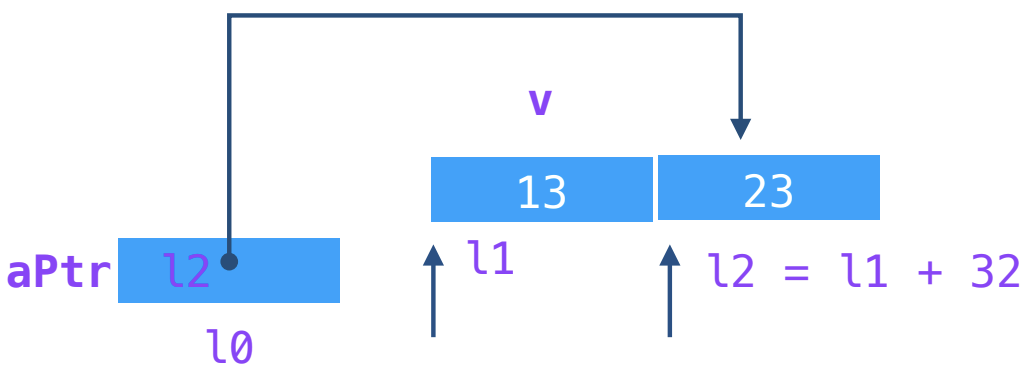
\includegraphics[width=7cm]{images/esempio-puntatori-1.png}
    \caption{Operazioni algebriche su puntatori}
\end{wrapfigure}

$\rho = [(aPtr, l2)]$ \: \: $\sigma = [(l1,13), (l2,23)]$\\ \\
Abbiamo quini un puntatore "aPtr" che punta alla locazione l1, il quale contiene il numero 13, più una posizione l2, successiva alla l1, che contiene 23.\\ Se ipotizziamo che il nostro sistemi archivi le informazioni con una base di 32 bit \footnote{Questo vuol dire che ogni vaore è salvato con 32 bit, quindi ogni 32 ci sarà un nuovo valore archiviato} ed andiamo a sommare 32 a "aPtr" succederà che ci sposteremo di 32 posti nella memoria raggiungendo l2, quindi "aPtr" = l2.

\subsection{Strutture dati}
\begin{definition}[Struttura dati]
Una \textbf{struttura dati} è un formato che serve ad organizzare e memorizzare dati in modo da renderli agevolmente disponibili agli algoritmi che li manipolano.
\end{definition}
\hspace{-15pt}Alcune caratteristiche delle strutture dati:
\begin{itemize}
    \item Una struttura dati è detta \textbf{omogenea} se contiene dati tutti dello stesso tipo. Altrimenti è \textbf{disomogenea}.
    \item Una struttura dati è \textbf{statica} se la sua dimensione non varia durante l'esecuzione del programma. Altrimenti è detta \textbf{dinamica}.
    \item Una struttura dati è \textbf{lineare} se i dati sono organizzati come sequenze di valori. Altrimenti è detta \textbf{non lineare}.
\end{itemize}
Una struttura dati è inoltre caratterizzata dalle operazioni elementari disponibili per inserire, reperire e modificare i dati che memorizza.
